
\section{Hardware}

	A major component of the project was discovering what was available in the industry.  This included finding what hardware was available to support Virtual and Augmented Reality.  The goal was to find what was existing to develop the platform requested by the clients.  Exploration was performed on Virtual Reality (VR) and Augmented Reality (AR) devices.  The following sections will summarize the research, including:

	\begin{itemize}
		\item What is AR and VR
		\begin{itemize}
			\item Differences between AR and VR
			\item Differences in hardware in each category
			\item Requirements to run the hardware
		\end{itemize}

		\item Web Technologies
		\item File Conversion
		\item Mobile Devices
	\end{itemize}
	
	It is important to remember that this section of the industry is rapidly developing.  What is presented in this document in May 2018 may be dated information shortly after.  Therefore, this research reflects the state of the technology from Fall 2017 to Spring 2018.

	
\subsection{Virtual and Augmented Reality}


    Virtual Reality (VR) is one of the fields explored during the development of the project.  VR headsets are designed to be fully immersive, so that the real world is blocked out in favor of the virtual.  This is different than AR where virtual objects are placed into the real world.  VR usually includes a headset tethered to a computer, tracking sensors placed in the room, and controllers.  On the other hand, AR devices usually rely on hand gestures to control the programs.

	% Research / Hardware / VRAR / VRDevices

\subsubsection{VR Devices}

	Currently (as of May 2018) there are two leading VR headsets: the Oculus Rift and HTC Vive.  The HTC Vive comes in two main forms, the regular Vive and the Vive Pro.  The Vive Pro is a wireless version of the Vive that has better specifications than the regular version.  The Vive sells for around \$500 and the Vive pro for \$800. The Oculus Rift (or Oculus for short) is produced by Facebook and sells for around \$400.

	\paragraph{HTC Vive}

		The HTC Vive is produced by HTC (headquartered in Taiwan).  It is considered the higher tier device (over the Oculus) but also has a higher price tag.  It heavily relies on the SteamVR software produced by Valve.  Tracking for the Vive is done using two "Lighthouses" placed in opposite corners of the room.  They work with the headset and controllers to determine where and what orientation the devices are in.  The information is then sent to the computer and displayed in the application.  The Vive software is heavily integrated with the SteamVR software.  SteamVR is Valve's integration with their popular gaming platform Steam.  It allows users to access their Steam account from within the VR setting to access the store, message friends, and play games.  The connection to the Vive takes place from the headset to a provided "Link box", and from the link box to the computer.  Overall the ports required on the computer are: 1 USB and 1 HDMI.

	\paragraph{Oculus Rift}

		As stated before, the Oculus is produced by Facebook (headquartered in California).  It is a cheaper option compared to the Vive.  It uses its own software to run the headset, but can use SteamVR.  Tracking is performed using two sensors that are placed on either side of the user's computer.  They each take up a USB 2.0 port. Overall, the setup takes 3 USB ports (2x 2.0, 1x 3.0) and 1 HDMI port.


    % Research / Hardware / ARDevices

\subsubsection{AR Devices}

	Augmented Reality devices are different than VR Devices in that the applications are presented on top of what the user would normally see, not blanking out the screen and recreating the world.  Currently, there are two main headset contenders in the AR space, Microsoft's HoloLens and the Meta 2.  Mobile devices are now becoming more popular for AR.

	\paragraph{HoloLens}

		The HoloLens is a wireless AR headset developed by Microsoft.  The developer edition of the HoloLens was released in March 2016, and has not had any further releases since.  They (Microsoft) are currently developing the HoloLens 2, the next iteration of the hardware.  The original version has some user complaints such as a small viewing port, that will be addressed in version two.  

	\paragraph{Meta 2}

		The Meta 2 is another headset.  It is wired, so a computer on par with the requirements for the Oculus VR headset is required.  Being wired is a downside for mobility, in that the user must always be close to a computer.  However, it is also a good thing in that the headset can use the more powerful processing on the computer rather than having the chips on board the headset.

	\paragraph{Mobile Phone}

		AR has recently been moving to the mobile phone space.  Both iOS and Android have AR offerings, ARKit and ARCore respectively.  ARKit was released by Apple in December 2017, and ARCore was released by Google in February 2018.  Since the offerings are so new, the number of applications developed with AR is still limited.  
		
		Mobile devices potentially have a larger consumer base than the dedicated headsets.  Most people have a smart phone (almost all running iOS or Android), and if AR was enabled on those devices, a large portion of the population would have AR capabilities.  Also, the mobile devices are more portable than the dedicated headsets.  A mobile phone can be carried in a pocket or small bag while the headsets must either be worn or be carried in a specialized carrying case.  
		
		One main drawback on running AR through mobile phones is the limited computational power.  A dedicated headset can have specialized hardware (including increased graphics processing) as opposed to a phone.  Also, all of the software on the headsets is designed for AR use.  So the user interfaces are designed with AR in mind, which may or may not be the case for the mobile devices.

    \subsubsection{Thoughts on Purchased Devices}

    A Microsoft HoloLens, Meta 2, and Oculus Rift were purchased by the client and available for testing and exploration via student status of developers. The following notes are observations made regarding these AR or VR hardware options.

    \begin{description}
        \item Microsoft HoloLens
            \begin{description} 
                \item Pros
                \begin{itemize}
                    \item Screen sharing over wireless internet  
                    \item Ability to record AR view and output to video
                    \item Hardware independence
                    \item Ability to statically place objects in environment
                    \item Support for most AR file types
                \end{itemize}
            \end{description}
            \begin{description} 
                \item Cons
                \begin{itemize}
                    \item Most expensive AR device on market
                    \item Portability plus value creates concern of theft
                    \item Limited AR display size
                    \item Limited availability of applications and support
                \end{itemize}
            \end{description}
        \item Meta 2
            \begin{description} 
            \item Pros
            \begin{itemize}
                \item Largest AR display size on market
                \item AR and VR capable
            \end{itemize}
        \end{description}
        \begin{description} 
            \item Cons
            \begin{itemize}
                \item Hardware dependent
                \item Limited availability of applications and support
            \end{itemize}
        \end{description}
        \item Oculus Rift
            \begin{description} 
            \item Pros
            \begin{itemize}
                \item Immediate availability of supplementary educational programs
                \item Most economic VR device (current market price of \$400)
                \item Intuitive controls
            \end{itemize}
        \end{description}
        \begin{description} 
            \item Cons
            \begin{itemize}
                \item VR only (no support for QR code use or real world visualizations)
                \item Hardware dependent
                
            \end{itemize}
        \end{description}
        \end{description}
	% Research / Hardware / PC

\subsection{PC}
	
%add section header to first included page

% \hypertarget{mobile_CodeDocumentation}
% {
%     \label{mobile_CodeDocumentation}
%     \index{mobile_CodeDocumentation@CodeDocumentation}    
% }
    
    
    
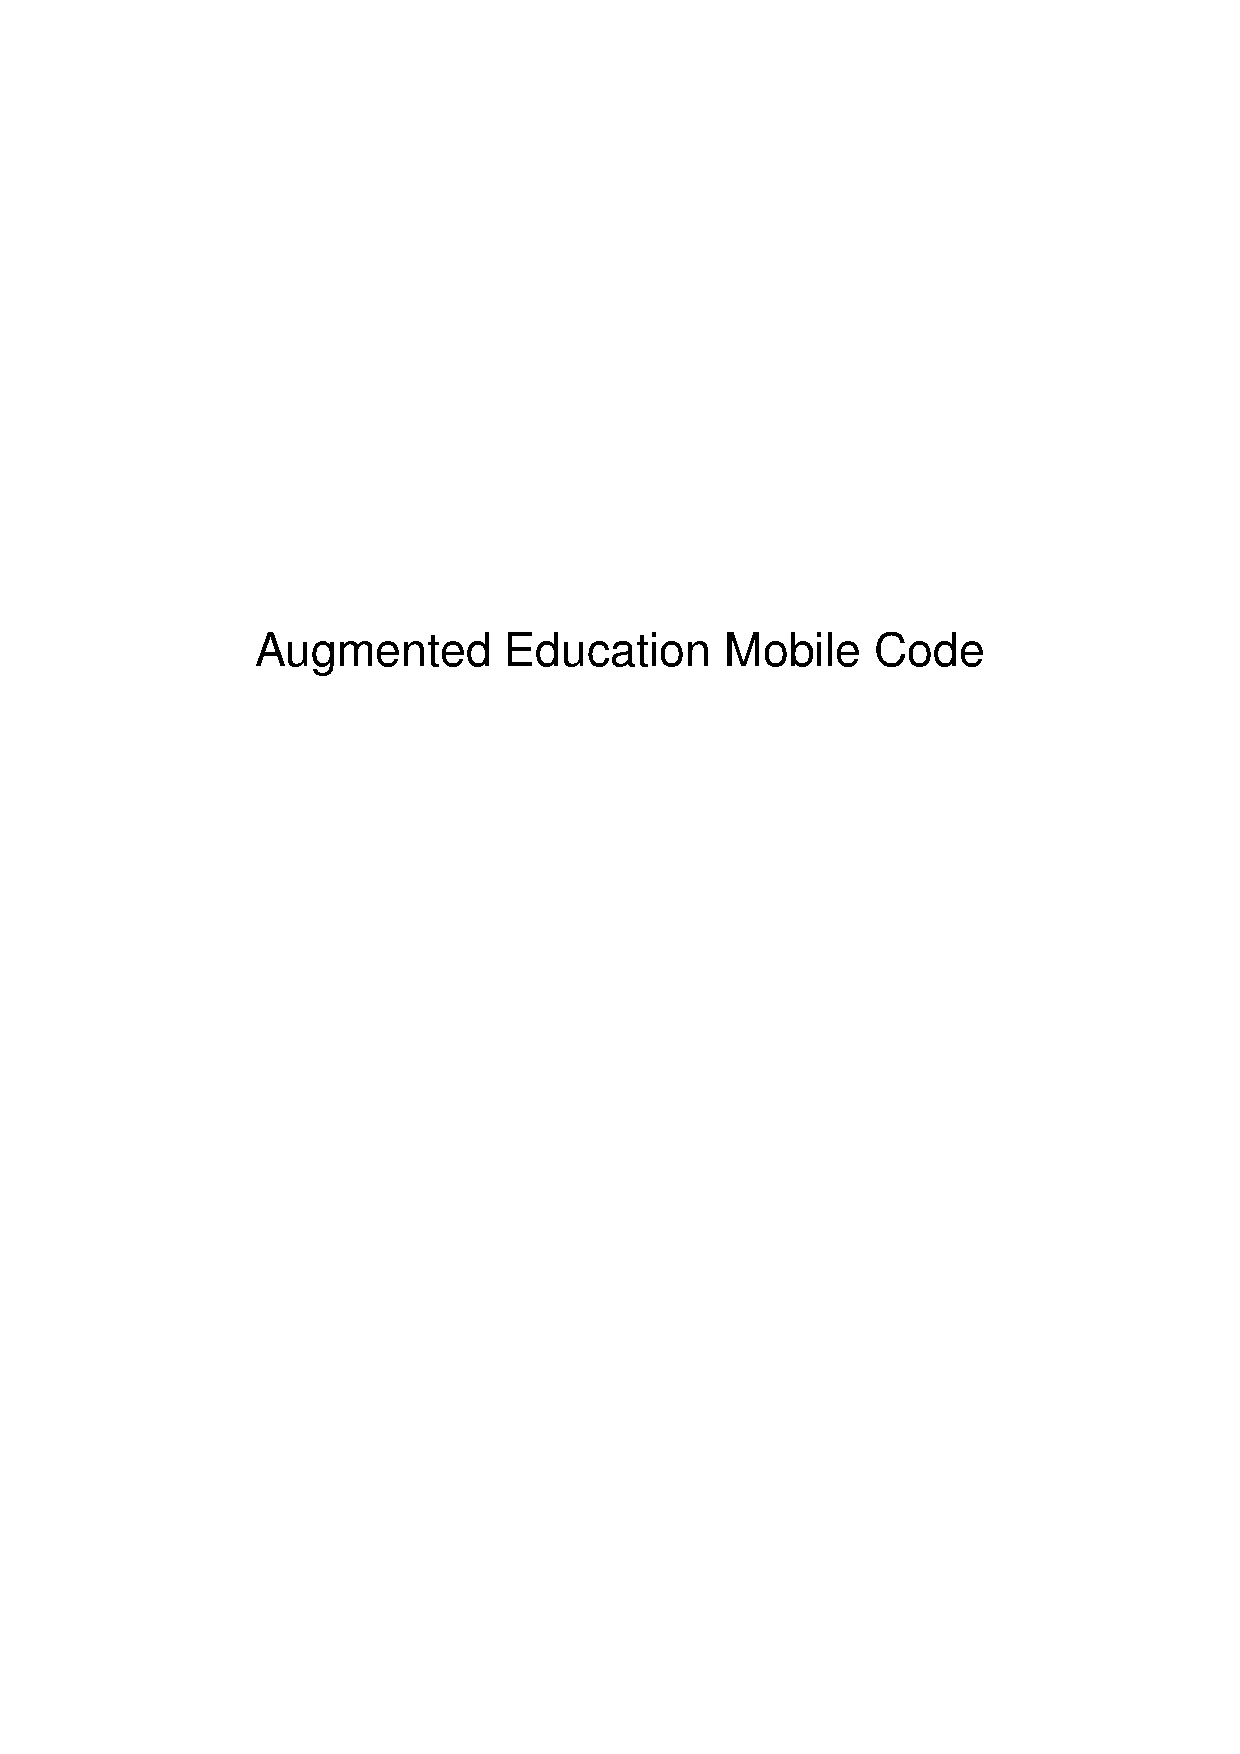
\includepdf[pages={1}, pagecommand=\section{Mobile Application}\hypertarget{mobile_CodeDocumentation}{\label{mobile_CodeDocumentation}\index{mobile_CodeDocumentation@CodeDocumentation}}]{CodeDocumentation/MobileCodeDoc}
\includepdf[pages={2-}]{CodeDocumentation/MobileCodeDoc}